\documentclass[11pt]{article}

\usepackage[margin=1.0in]{geometry}
%\linespread{1.5}
\usepackage{graphicx}
\usepackage{natbib}
\usepackage{amsmath}
\usepackage{fancyhdr}
\usepackage{changepage}
\usepackage{rotating}
\sloppy

\pdfminorversion 4

\bibpunct[,]{(}{)}{;}{a}{}{,}


\renewcommand{\bottomfraction}{.9}
\renewcommand{\topfraction}{.9}
\renewcommand{\textfraction}{0.1}
\renewcommand{\floatpagefraction}{.9}




\fancypagestyle{plain}{%
   \fancyhead[R]{\fbox{\big{\textbf{Letter}}}}
   \renewcommand{\headrulewidth}{0pt}
}


\begin{document}

\title{\textbf{Limited utility of residue masking for positive-selection inference}}
\author{Stephanie J. Spielman$^{1*}$ and Eric T. Dawson$^{1}$ and Claus O. Wilke$^{1}$}
\date{}

\maketitle
\noindent
Address:\\
$^1$Department of Integrative Biology, Center for Computational Biology and Bioinformatics, and Institute of Cellular and Molecular Biology.
The University of Texas at Austin, Austin, TX 78712, USA.\\

\bigskip
\noindent
$^*$Corresponding author\\
$\phantom{^*}$Email: stephanie.spielman@utexas.edu\\

\bigskip
\noindent
Manuscript type: Letter

\bigskip
\noindent Keywords: multiple sequence alignment, alignment filters, positive-selection inference, sequence simulation

\newpage
\begin{abstract}
Errors in multiple sequence alignments (MSAs) can reduce accuracy in positive-selection inference. Therefore, it has been suggested to filter MSAs before conducting further analyses. One widely-used filter, Guidance, generates site-specific MSA confidence scores, allowing users to remove positions of low confidence. However, while some have found that Guidance substantially improves accuracy in positive-selection inference, others have found that filtering affects accuracy only minimally. Motivated by this discrepancy, we have conducted an extensive study to characterize how Guidance impacts positive-selection inference. We particularly investigated whether novel scoring algorithms, which phylogenetically corrected confidence scores, and a new gap-penalization score-normalization scheme improved Guidance's performance. We found that no filter, including original Guidance, consistently improved inferences. Moreover, all improvements detected were exceedingly minimal, and in certain circumstances, Guidance worsened inferences.
\end{abstract}



Multiple sequence alignment (MSA) construction represents the most fundamental step nearly all molecular evolution studies. Recently, several studies have shown that poor MSA quality can hinder accuracy in positive-selection inference \citep{Schneider2009, Fletcher2010, MarkovaRaina2011}. In response, some have advocated that users filter MSAs before subsequent analyses to remove putatively-poorly aligned regions \citep{Privman2012,Jordan2012}, thereby reducing noise and maximizing signal.

One widely-used filter, known as Guidance \citep{Penn2010}, derives a confidence score for each MSA position by sampling variants in guide trees when constructing progressive alignments. Users can then mask positions that score below a set threshold, thus removing residues contributing putatively misleading signal. Unfortunately, studies investigating Guidance's utility in positive-selection inference have produced conflicting findings. While one study \citep{Privman2012} found that Guidance dramatically improved accuracy, a separate study \citep{Jordan2012} found that Guidance affected positive-selection inference only modestly. Both studies found that filtering was primarily beneficial when sequences were highly diverged. Overall, \citet{Privman2012} strongly advocated Guidance's use, while \citet{Jordan2012} emphasized relying primarily on robust MSA construction methods. 

To reconcile these distinct recommendations, we have conducted an extensive simulation-based study to elucidate how the Guidance filter affects positive-selection inference, particularly for sequences of realistic divergence levels. We additionally examined the potential benefits to modifying the Guidance scoring scheme in several ways.  First, we assessed whether two novel algorithms that corrected Guidance scores for the sequences' phylogenetic relationships could improve upon the original Guidance algorithm. The first phylogenetically-corrected method incorporated a weight, calculated by BranchManager \citep{Stone2007}, for each MSA sequence, and the second method incorporated patristic distances (the sum of branch lengths between two taxa), calculated through the Python library Dendropy \citep{Sukumaran2010}. We refer to these methods, respectively, as BMweights and PDweights. Moreover, we tested a new gap-penalization score-normalization scheme, which scaled a given residue's score according to the number of gaps in its column, thus capturing the inherent unreliability of residues in gappy regions. We refer to filters using the gap-penalization scheme as GuidanceP, BMweightsP, and PDweightsP. To assess the performance of these novel algorithms, we reimplemented the Guidance software (available at https://github.com/clauswilke/alignment\underline{\hspace*{0.2cm}}filtering). 

We simulated protein-coding sequences using Indelible \citep{Fletcher2009} according to two different selective profiles: H1N1 influenza hemagluttinin (HA), which featured a mean $dN/dS = 0.37$, and HIV-1 envelope protein subunit GP41, which featured a mean $dN/dS = 0.89$. We used these selective profiles because, while both genes contain positively selected regions \citep{Bush1999, Frost2001, Bandawe2008, Meyer2012}, the majority of sites in HA are either under strong purifying or positive selection, whereas a relatively higher proportion of sites in GP41 have $dN/dS$ values closer to 1, making positive-selection inference more challenging. For each selective profile, we simulated 100 MSA replicates along each of four different gene trees consisting of 11, 26, 60, and 158 taxa, yielding a total of 800 simulated MSAs. All sequences were simulated with a 5\% indel rate, as is typical of mammalian genomes \citep{Cooper2004}. Trees were obtained from \citet{Spielman2013}, \citet{Yang2011}, and \citet{Betancur2013}.

We processed the unaligned amino-acid sequences with our Guidance reimplementation using the aligner MAFFT L-INS-I (linsi) \citep{Katoh2002,Katoh2005} and calculated confidence scores for all inferred MSAs using each of the six scoring algorithms. We masked all positions with scores below 0.5, the same threshold as used by \citet{Jordan2012}. We selected this threshold based on results which showed that a stringent threshold (e.g., 0.9 as used by \citealt{Privman2012}) had the potential to worsen selection inference in certain cases (see Supplementary Material, Table S1).

We infered positive selection using two methods: FUBAR \citep{Murrell2013}, implemented in HyPhy \citep{Pond2005}, and standard PAML M8 model \citep{Yang2000, Yang2007}. Phylogenies used during positive-selection inference were constructed in RAxMLv7.3.0 using the ``PROTGAMMAWAG" model \citep{Stamatakis2006}. While we processed all MSAs with FUBAR, we did not process the MSAs containing 158 taxa with PAML due to prohibitive runtimes. A detailed description of all methods, including the Guidance software reimplementation, is available in Supplementary Materials.


\subsection*{Guidance-based filters have a minimal effect on positive-selection inference}

We first compared the resulting true positive rates (TPRs) of positive-selection inference between each filtered MSA and its corresponding unfiltered MSA. We chose to primarily compare the TPRs, as opposed to the false positive rates (FPRs), as the FPRs we recovered were exceedingly small, never surpassing an average of 1\% across simulation sets and inference methods. TPRs were calculated using the true evolutionary rates assigned during sequence simulation. For this analysis, we considered sites to be positively selected if the given inference method (i.e. FUBAR or PAML) returned a posterior probability $\geq0.90$. For each simulation set, we fit a series of mixed-effects models using the R package lme4 \citep{Bates2012}. Each model contained TPR as the response variable, filtering algorithm (including no filtering) as a fixed effect, and simulation count as a random effect.

Table \ref{tab:summarystats} summarized our main results. We generally found that all filters within a given normalization scheme performed statistically indistinguishably. Therefore, Table \ref{tab:summarystats} displays results for only Guidance and GuidanceP (Table S2 contains results for all filters). Table \ref{tab:summarystats} demonstrates that, for the majority of simulation sets, Guidance-based filtering did not significant affect TPR. While MSA filtering significantly increased mean TPR in a few cases, filtering also significantly decreased mean TPR in other cases. Even so, all statistically significant effects were of extremely small magnitudes. Interestingly, we also found that GuidanceP provided both the largest TPR increases and the largest TPR decreases, while Guidance performed more consistently, only significantly reducing TPR in one case. Additionally, Guidance influenced mean TPR more modestly and less frequently than GuidanceP.

Moreover, inference methods responded inconsistently to filtered MSAs, as demonstrated in Figure~\ref{barplot}, which gives a graphical representation of the linear models' results for the 26- and 60-sequence simulation sets. On one hand, filters had similar behavior across simulation sets when analyzed with FUBAR (Guidance TPR was generally higher than were both unfiltered and GuidanceP), but this trend was mostly statistically insignificant. Alternatively, filters did not behave consistently across simulation conditions when analyzed with PAML. For instance, the HA 26-sequence simulation set, when processed with GuidanceP and PAML, exhibited the largest TPR improvement in this study. However, GuidanceP also significantly reduced mean TPR for the GP41 60-sequence simulation set, also as inferred with PAML. 

In sum, it was difficult to identify clear trends dictating whether filtering improved or hindered accuracy. However, we emphasize that all Guidance-based filters improved positive-selection inference for both 158-taxa simulation sets, although effect magnitudes were miniscule. As we did not analyze these data sets with PAML, we caution this result may not be easily extrapolated to inference methods other than FUBAR. Additionally, all filters significantly reduced accuracy for the GP41 11-sequence simulation set as analyzed with PAML. Thus, we did recover a slight trend suggesting that MSA filtering should be reserved for larger MSAs.

\subsection*{Guidance-based filters improve power under narrow conditions}

We additionally used receiver operating characteristic (ROC) curves to qualitatively assess whether MSA filtering influences power in positive-selection inference. Importantly, this analysis did not bias results to those obtained from a single posterior probability threshold for calling positive-selected sites. ROC curves for the HA and GP41 60-sequence simulation sets are shown in Figure~\ref{roc}. 

Several trends emerge from Figure~\ref{roc}. First, power in positive-selection inference for HA simulation sets was universally greater than for GP41 simulation sets. Given that the GP41 sequences featured a greater proportion of sites with $dN/dS$ near 1, this result was unsurprising. Second, as all algorithms within a given normalization scheme (original vs. gap-penalization) had nearly identical curves, this analysis confirmed that introducing phylogenetically-weighted scores did not strongly affect Guidance scores. Finally, across the entire span of the ROC curves, no dramatic difference in area between unfiltered and filtered MSA curves existed, although, MSAs filtered with gap-penalization algorithms did, at certain FPR levels (roughly 0.1--0.3), perform worse worse than did both unfiltered and Guidance-filtered MSAs. 

However, filtering did substantially increase power at very low FPR rates, as seen in the right-hand panels, in particular when using PAML. These benefits, unfortunately, only existed at FPR levels of roughly 1\% - 4\%, above which any improvements quickly dissipated. Outside of this 1-4\% FPR region, filtered MSAs either performed the same as or worse than unfiltered MSAs.
Importantly, when we identified positively-selected sites at a posterior probability $\geq 0.9$, all recovered FPRs were, on average, less than 1\%, below the region where filtering increased power. Our low recovered FPRs explained why we did not detect substantial benefits to MSA-filtering through our linear models. Taken together, these results demonstrated that Guidance-based filtering was not robust to varying FPR levels. ROC curves for all other simulation sets are available in Figures S1 and S2, and yielded results broadly consistent with those described here.

\subsection*{Discussion and Conclusions}

The primary goal of using the Guidance, or similar, MSA filters is to remove excessive noise while maintaining informative data. Ideally, our study would have recovered a clear set of circumstances for which Guidance-based filters could consistently achieve this goal. Instead, we recovered few conditions for which filtering strictly removed noise but preserved signal. Guidance-based filtering was most useful for FPR levels ranging from 1-4\%, but in any given study it is impossible to know if the data actually fall in this range. If the data fall outside of this range, there appears to be substantial risk of lowering power.

Our study focused primarily on divergence levels representative of realistic protein-coding data typically used in positive-selection inference. Therefore, it is possible that Guidance would have provided stronger benefits with highly diverged data \citep{Privman2012}. However, as seen in Table \ref{tab:summarystats}, our MSAs contained gaps in up to 60\% of columns, meaning that constructing MSAs on our datasets was not a trivial task, and portions which were difficult to align certainly existed (Table S2).

We additionally found that, for nearly all simulation cases, FUBAR outperformed PAML both in TPR and runtime. Each FUBAR inference completed in under 20 minutes, but a single PAML inference took between two hours and a week to complete. FUBAR, therefore, represents a fast and accurate alternative to traditional positive-selection inference methods.

In sum, two distinct conclusions may be drawn from our study. First, although Guidance did not universally benefit positive-selection inference, it never entirely precluded detection of positively-selected sites. Therefore, filtering could be used as a conservative method in selection inference. Second, all benefits that filtering conferred were minimal, and filters behaved inconsistently across simulation sets and inference methods. Given these observations, there is no guarantee that MSA filtering will help or harm any given analysis. In fact,  Guidance filtering may inadvertently result in a loss of power. 

We conclude that, while potentially beneficial, Guidance-based filtering is not a particularly robust method for positive-selection inference, and therefore does not need to be a necessary component of positive-selection studies. Finally, we recommend that users primarily focus on employing high-quality MSA inference (e.g. linsi \citep{Katoh2005} or PRANK \citep{Loytynoja2008}) and positive-selection inference (e.g. FUBAR) methods, in which error can be minimized as much as possible preserve informative signal. Should users opt to filter their MSAs, we recommend using a lenient cutoff ($\leq0.5$) to preserve informative signal.


\subsection*{Supplementary Material}
Supplementary methods, Figures S1 and S2, and Tables S1, S2, and S3, are available at Molecular Biology and Evolution online (http:// www.mbe.oxfordjournals.org/).


\subsection*{Acknowledgements}
 This work was supported in part by ARO grant W911NF-12-1-0390, NIH R01 GM088344, and NSF Cooperative Agreement No. DBI-0939454 (BEACON Center). The authors thank Eyal Privman for constructive discussion and Sergei Kosakovsky Pond for valuable  comments, for providing a GP41 alignment and phylogeny, and for help using FUBAR.


\bibliographystyle{MBE}
\bibliography{citations}	

\newpage

\begin{table}[htbp]
\begin{adjustwidth}{-1cm}{}
\caption {\label{tab:summarystats} Summary statistics for effect of masking.}
\begin{tabular}{l l l c c c c c}
\hline\noalign{\smallskip}
& & & \multicolumn{4}{c}{Mean True Positive Rate} \\
\cline{4-7}\noalign{\smallskip}
\multicolumn{1}{p{1.5cm}}{\centering Selective \\ Profile} & \multicolumn{1}{p{1.5cm}}{\centering Number \\ of Taxa} & \multicolumn{1}{p{1.5cm}}{\centering Inference \\ Method} & \multicolumn{1}{c}{True} & \multicolumn{1}{c}{Unfiltered} & \multicolumn{1}{c}{Guidance} & \multicolumn{1}{c}{GuidanceP} & \multicolumn{1}{c}{Percent Gaps} \\
\noalign{\smallskip}\hline\noalign{\smallskip}
HA  &  11  &  FUBAR  &  0.093  &  0.084  & 0.085 (1.33\%)  &  0.085 (0.74\%) & 11.9\% \\
  &    &  PAML  &  0.086  &  0.082  & 0.081 (-0.48\%)  &  0.081 (-0.60\%) &\\

 & 26 & FUBAR & 0.252 & 0.227 & 0.229 (0.84\%) & 0.226 (-0.38\%) & 26.0\%\\
 &   & PAML & 0.209 & 0.176 & \textbf{0.178 (1.36\%)$^{\ast\ast}$} & \textbf{0.183 (4.04\%)$^{\ast\ast}$} &\\

 & 60 & FUBAR & 0.551 & 0.474 & 0.479 (0.99\%) & \textbf{0.464 (-2.16\%)$^{\ast}$} & 59.4\%\\
 &  & PAML & 0.422 & 0.347 & 0.342 (-1.68\%) & 0.337 (-2.92\%) &\\

 & 158 & FUBAR & 0.515 & 0.458 & \textbf{0.467 (1.89\%)$^{\ast}$} & \textbf{0.468 (2.12\%)$^{\ast}$} & 50.5\%\\
\noalign{\smallskip}\hline\noalign{\smallskip}
GP41  &  11 &  FUBAR  &  0.062  &  0.058  &  0.057 (-1.55\%)  &  0.057 (-1.21\%) & 11.6\%\\
  &    &  PAML  &  0.096  &  0.098  & \textbf{0.095 (-3.49\%)$^{\ast\ast}$}  &  \textbf{0.095 (-3.80\%)$^{\ast\ast}$} &\\

 & 26 & FUBAR & 0.216 & 0.196 & \textbf{0.20 (1.89\%)$^{\ast}$} & 0.197 (0.36\%) & 31.3\%\\
 & & PAML & 0.237 & 0.216 & 0.220 (1.54\%) & 0.217 (0.244\%) &\\

 & 60 & FUBAR & 0.359 & 0.308 & \textbf{0.313 (1.77\%)$^{\ast}$} & 0.304 (-1.16\%) & 58.1\%\\
 & & PAML & 0.341 & 0.304 &0.302 (-0.77\%) & \textbf{0.296 (-2.71\%)$^{\ast\ast}$} & \\

 & 158 & FUBAR & 0.348 & 0.320 & \textbf{0.325 (1.77\%)$^{\ast\ast}$} & \textbf{0.326 (2.02\%)$^{\ast\ast}$} & 48.4\% \\
\noalign{\smallskip}\hline\noalign{\smallskip}
\end{tabular}
\newline
\textsc{note.}--- Mean TPR values shown in bold represent those which are significantly different from the respective unfiltered MSA mean TPR. Values shown in parentheses refer to the average TPR percent change of the respective unfiltered MSA, not the absolute TPR increase or decrease. Significance levels:  $^{\ast\ast} P < 0.001$; $^{\ast} P < 0.01$. All significance levels were corrected for multiple comparisons using the R multcomp package \citep{Hothorn2008}. Note that the true MSAs were not included in the linear models but are shown here for comparative purposes. Percent gaps were calculated from unfiltered alignments as the total number of gaps divided by the total number of MSA positions, and represent the percentage of columns with at least one gap, averaged across all MSA replicates.
\end{adjustwidth}
\end{table}

\begin{figure*}[H]
\centerline{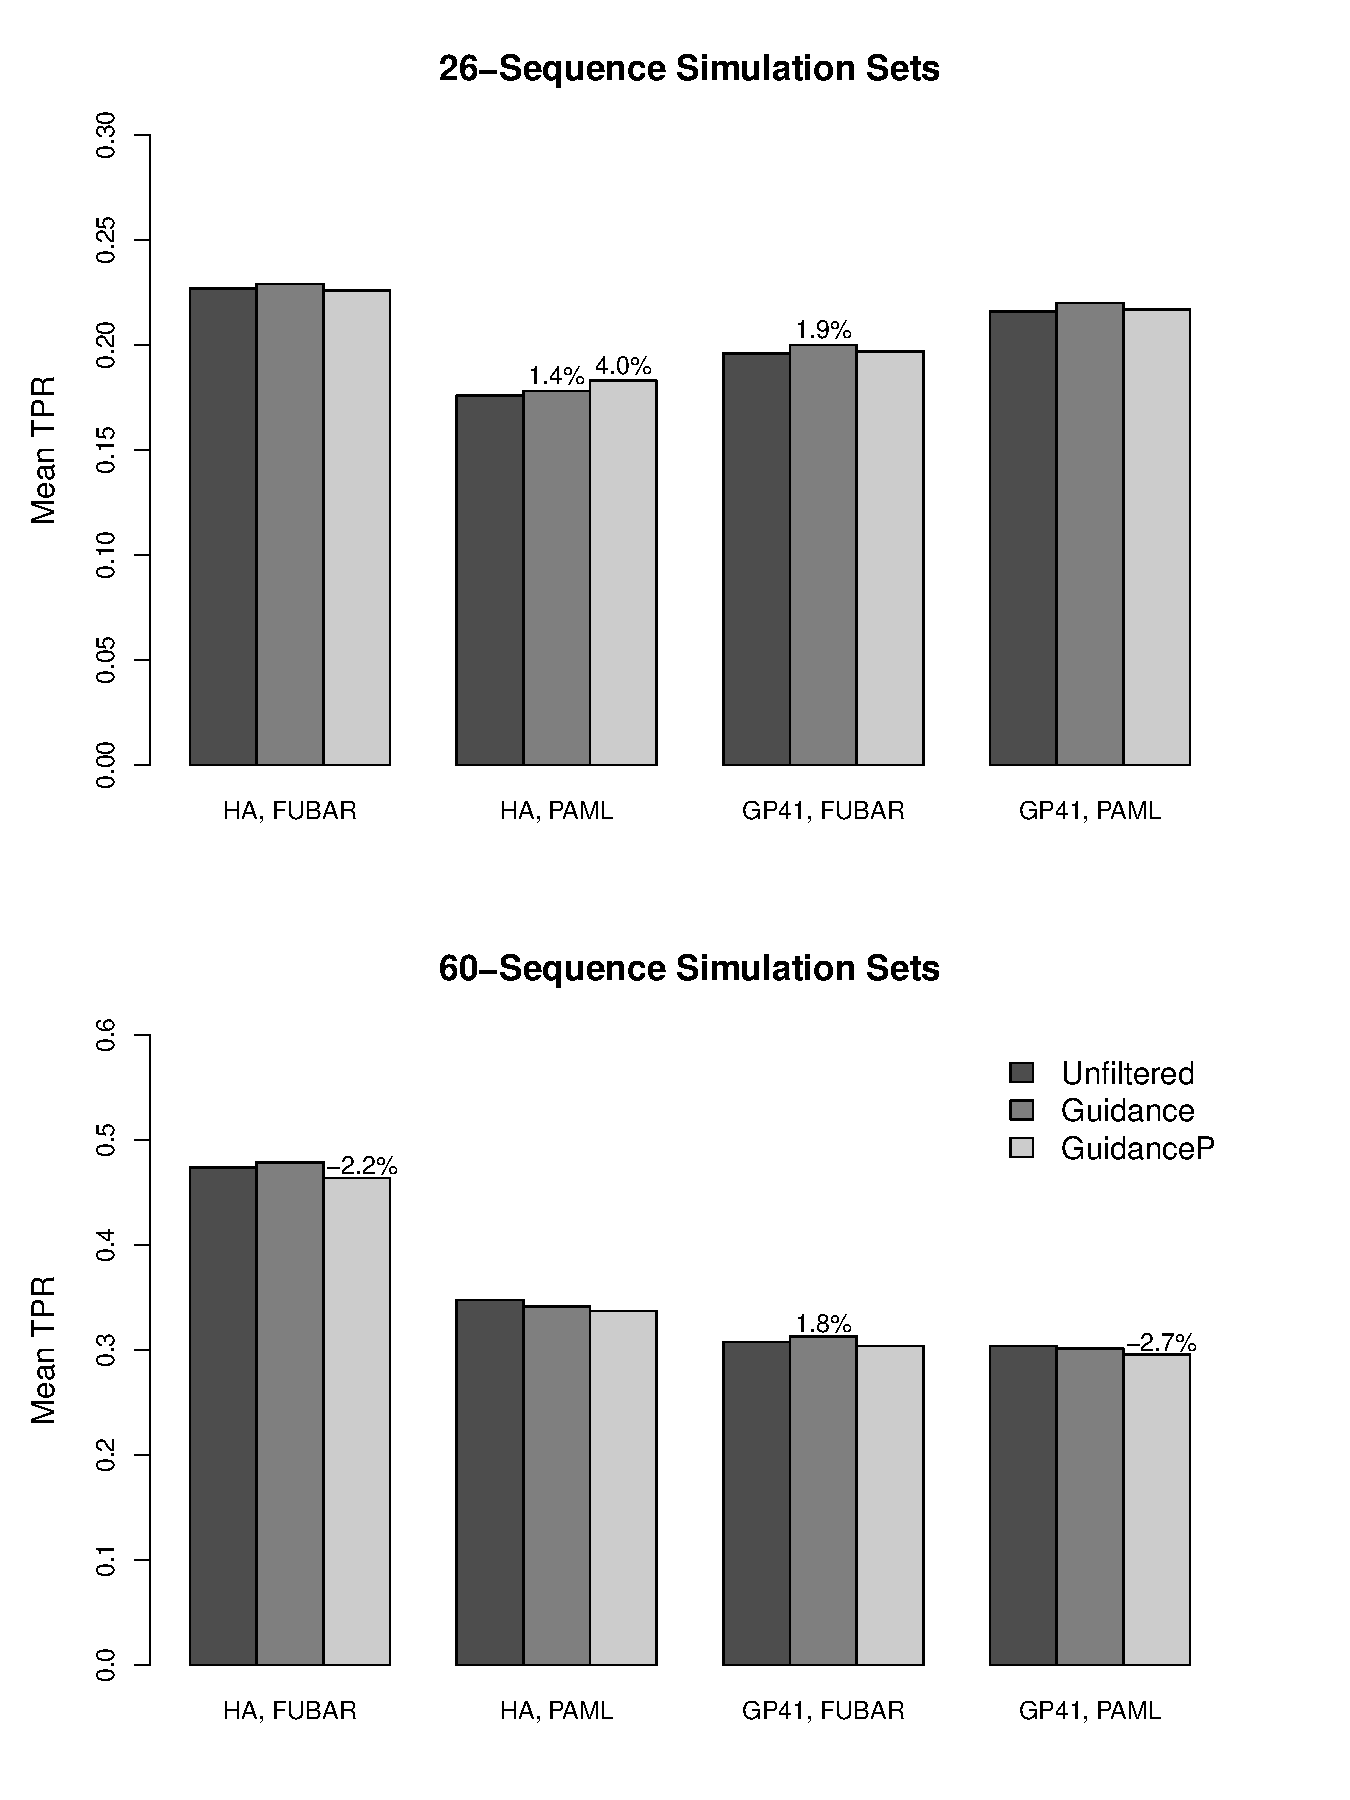
\includegraphics[width=4.75in]{Figures/barplot.pdf}}
\caption{\label{barplot} Mean TPR for and 26- and  60-sequence simulation sets. Percentages, which represent the average percent TPR change relative to the unfiltered MSAs, are shown only for those changes which are significant. Significance levels are the same as those given in Table \ref{tab:summarystats}. (A) Simulations with 26 sequences. (B) Simulations with 60 sequences.}
\end{figure*}

\bigskip

\begin{figure*}[H]
\centerline{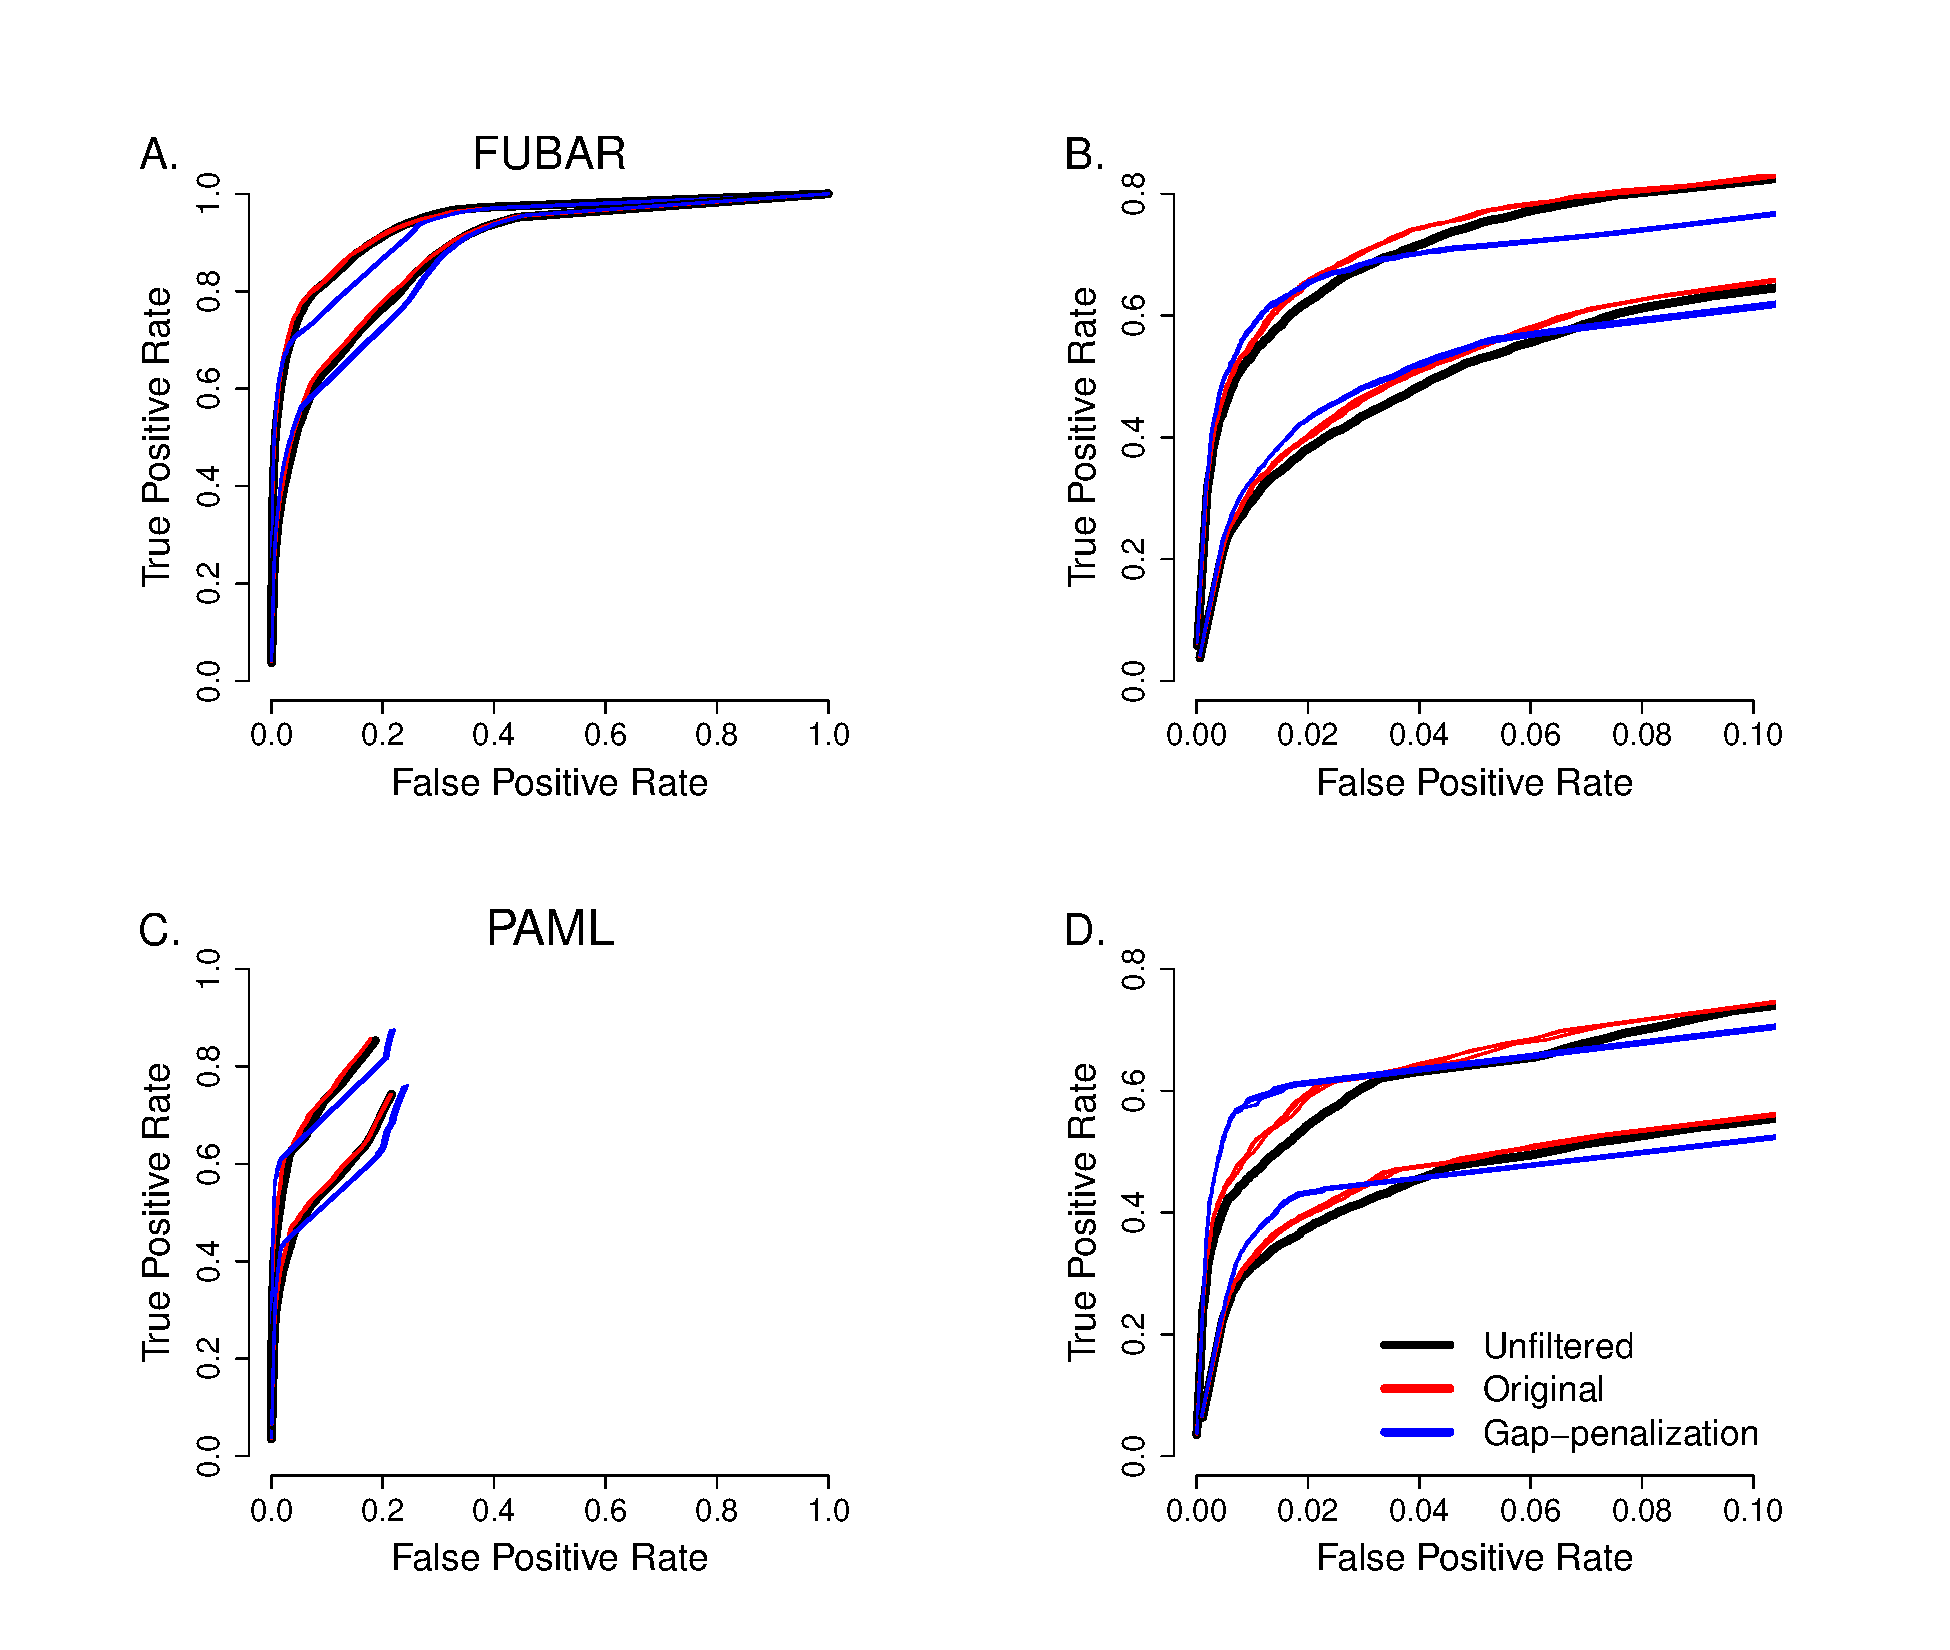
\includegraphics[width=6in]{Figures/ROC_prk.pdf}}
\caption{\label{roc} ROC curves as averaged across the two 60-sequence simulation sets. Within each panel, the top curve represents results from the HA selective profile, and the bottom curve represents results from the GP41 selective profile. Full ROC curves are shown in the left-hand panels. Note that, for the full PAML ROC curves, average FPRs higher than shown were not seen. The right-hand panels highlight specifically the low FPR regions (0--0.1) of the ROC curves. All MSA filtering algorithms (Guidance, BMweights, PDweights, GuidanceP, BMweightsP, and PDweightsP) are shown in ROC curves. (A-B) ROC curves for positive-selection inference by FUBAR. (C-D) ROC curves for positive-selection inference by PAML M8.}
\end{figure*}

\end{document}